\chapter{設計}\label{chap:design}

本章ではその場に居合わせた人達の情報共有を可能にするサービスアプリケーションの設計について述べる。

\newpage

\section{アプリケーションの設計}

ここでは、その場に居合わせた人々が効率的に情報共有を行うためのアプリケーション、および周辺のシステムの設計について述べる。


\subsection{その場に居合わせていることへの保証}

ユーザが持っている近くに居るというコンテキストを判定するには、
第\ref{chap:background}章で述べたとおり、いくつかの手法が挙げられる。
確実にその場にいる人達との情報共有手法として、
Bluetoothによる近接デバイスの検出は適していると言える。
本アプリケーションでは、一般的なモバイルデバイスの持つBluetoothモジュールを利用した近接デバイス検出機能により、
その場に居合わせている人間の探索を実現する。


\subsection{情報の不揮発性}

本アプリケーションで共有された情報は、
発信地であるその場を離れても、受け取った人間が後で見返したり、
別の場所に共有することを可能とすることを目的としている。
そのためには、情報がその場限りで消えてしまうような揮発性を持ってはいけない。
情報の発信源である元のデバイスが近接する場所から離れても、
共有された情報は見られるように保存されるべきである。

アクティビティはアプリケーションがインストールされているデバイスに保管、
またはデータにアクセスできるよう保存され、
投稿された情報やメディアは後から見返せるようにする必要がある。

そのため、やりとりされる情報はMANETのような閉鎖的なネットワーク内でやりとりするのではなく、
全てWeb上に生成され、ブラウザ上から見られる方式が適していると考える。


\subsection{本人到達性とリンク可能性}

情報共有のサービスにおいては、
共有される情報とそれに結び付いた付加的な情報(発言者、時刻など)をどのように表現するかによって、
交わされる情報の内容が変化する。

例えば、発信者の本名および個人情報と結びついた情報ならば、
情報の内容は公共の場での発言と遜色のないものとなるだろう。
逆に匿名ならば、2ちゃんねる\cite{2ch}などに見る自由な発言内容が見られるだろう。

匿名性を測る指標として、本人を特定する本人到達性と、
表示されている投稿などが同一人物であるか判定するリンク可能性という、
2つの要素があると言われている。\cite{anon_terminology}

また、社会心理学の分野の研究\cite{diet}では、匿名性による社会的手がかりの減少から、
偏見やステレオタイプが避けられ、自己開示が促進されるメリットとともに、
共有された話題がテーマの場合は、情報に対する信頼度が十分に保たれるという結果が出ている。

\begin{figure}[h]
    \begin{center}
        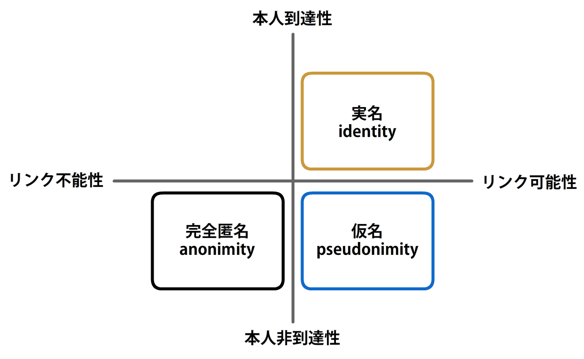
\includegraphics[width=0.8\linewidth]{img/anon.eps}
    \end{center}
    \caption{本人到達性とリンク可能性}
    \label{fig:anon}
\end{figure}

同じ場所に居合わせた見知らぬ人同士にとっては、情報開示に対するプライバシーの意識は敏感な問題である。
そのため、活発な情報開示を促進するために、匿名性を有するインターフェイスを提供する必要があると考える。

アプリケーションでは、リンク可能性を維持しながら、
本人到達性を減少させることで、仮名(pseudonym)によるサービスの設計を目指す。
